\section{Paralelogramo}

\begin{frame}[fragile]{Definição de paralelogramo}

    \begin{itemize}
        \item Um paralelogramo é um quadrilátero cujos lados opostos são paralelos

        \item Além do retângulo e do quadrado, outro paralelogramo notável é o losango

        \item O losango é um paralelogramo cujos lados opostos são iguais

        \item Porém seus ângulos internão não são necessariamente iguais

        \item Um paralelogramo pode ser caracterizado ou pelas coordenadas de seus
            vértices ou pelas medidas dos lados adjacentes ($a$ e $b$) e um de
            seus ângulos internos (os demais podem ser deduzidos a partir deste)
    \end{itemize}

    \begin{figure}
        \centering

        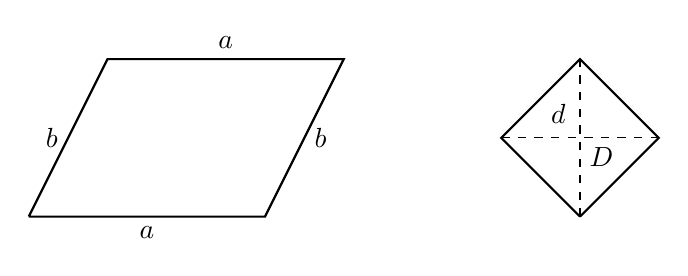
\begin{tikzpicture}
            \coordinate (A) at (0, 0);
            \coordinate (B) at (3, 0);
            \coordinate (C) at (4, 2);
            \coordinate (D) at (1, 2);

            \draw[thick] (A) -- node[anchor=north] { $a$ } (B) -- node[anchor=west] { $b$ } (C) -- node[anchor=south] { $a$ } (D) -- node[anchor=east] { $b$ } (A);

            \coordinate (A) at (7, 0);
            \coordinate (B) at (6, 1);
            \coordinate (C) at (7, 2);
            \coordinate (D) at (8, 1);

            \draw[thick] (A) -- (B) -- (C) -- (D) -- (A);

            \draw[dashed] (A) -- node[anchor=north west] { $ D $ } (C);
            \draw[dashed] (B) -- node[anchor=south east, inner sep=5pt] { $ d $ } (D);
        \end{tikzpicture}
    \end{figure}

\end{frame}

\begin{frame}[fragile]{Área e perímetro}

    \begin{itemize}
        \item O perímetro de um paralelogramo é igual ao dobro da soma das medidas de 
            seus lados adjacentes

        \item A área de um paralelogramo é dado pelo produto de sua base pela altura

        \item Em geral, é preciso determinar a altura, considerando um dos lados como base e 
            usando o ângulo formado com um dos lados adjacentes para montar um triângulo, onde a
            altura seria o cateto oposto ao ângulo

        \item No caso do losango, a área pode ser determinada diretamente se conhecidas as
            medidas das duas diagonais $D$ e $d$, denominadas diagonal maior e menor, 
            respectivamente

        \item Neste caso, a área é a metade do produto das diagonais, isto é,
        \[
            A = \frac{Dd}{2}
        \]

    \end{itemize}

\end{frame}
